%
%   K A D O N O
%   "kadono.tex"
%

\documentclass[10pt,b5paper,papersize,dvipdfmx]{jsbook}

\usepackage{vuccaken}
\usepackage{vuccaken2019}

% スタイルファイルの読み込みや自作マクロは、
% 最終的には vuccaken2019.sty の中に書いてください。
% とりあえずはここに書いてもらって構いません。


\begin{document} % 以下本文

\mokuji{2} % 目次出力

% - - - - - - - - - - - - - - - - - - - - - - - - %
\kaishititle%
  {固体中の熱}% title
  {物理科学 M1回生}% 所属
  {\vname{門野}{広大}}% name
% - - - - - - - - - - - - - - - - - - - - - - - - %

\section*{はじめに}
熱って何?温度ってなに?どうやって熱は伝わっているの?そんな疑問に一生に一度は出会ったことがあると思います。実際熱の伝わり方というものをちゃんと理解しようとすると莫大な時間がかかりますし、不可逆なものでもあるのでそもそも理解できないのかもしれません。でも、限定的な条件において理解することは容易にできます。今回の会誌ではそんな物理の世界では常識的なことを主に書いていきたいと思います。\par
今回は状況が限定的な状態で、実際に人間が住んでいる環境とはかけ離れているため役に立たないと思われると思います。研究分野ではとても役にたちます。その理由を最後の方に私がやっている研究の話を含めて書きたいと思います。

% 熱って何?そもそも温度って何?熱伝導率って何で決まるの?物質のなに?格子ってなに?
% 格子振動って何?フォノンってなに?

%
\section{温度}



\section{フォノン君}
固体中の熱物性を考えるに当たって固体がどういう構造になっているのかということをモデル化していく必要があります。まず簡単に一つの原子しかない単結晶の場合を考え、結晶中の原子同士がばねでつながっているモデルを考えます。図\ref{fig:bane}
\begin{figure}[htbp]
  \centering
  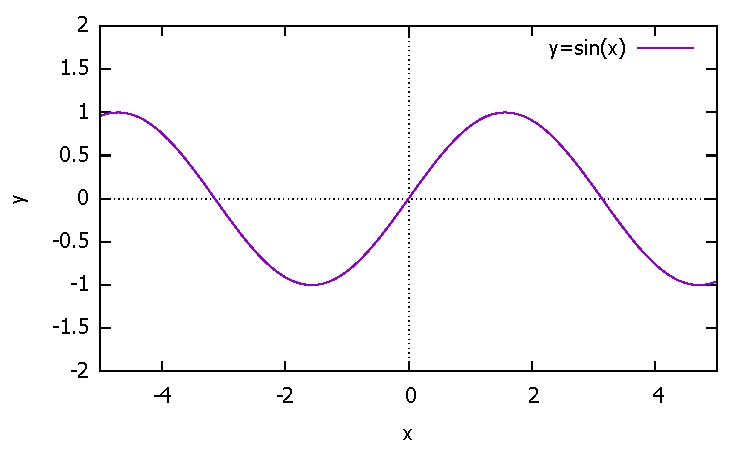
\includegraphics[width=10cm]{temp/fig-sin.pdf}
  \caption{一次元の結晶}
  \label{fig:bane}
\end{figure}

\section{比熱とか熱伝導率とか}

\section{ちょっと変わった話}

\section{終わりに}

%% 参考文献
\begin{thebibliography}{99}
<<<<<<< HEAD
    \item 横田伊佐秋 著 物理学テキストシリーズ 熱力学 岩波書店 (1987)
    \item W.COCHRAN 著 小林正一、福地充 訳 固体物性シリーズ3格子振動 丸善出版 (昭和50年)
    \item 田崎晴明 著 新物理学シリーズ37統計力学 培風館 (2008)
  \end{thebibliography}
=======
  \item 横田伊佐秋,『物理学テキストシリーズ 熱力学』,岩波書店,1987.
  \item W.COCHRAN・小林正一・福地充(訳),『固体物性シリーズ3 格子振動』,丸善出版,昭和50年.
  \item 田崎晴明,『新物理学シリーズ37 統計力学』, 培風館,2008.
\end{thebibliography}
>>>>>>> 5dd157f06b54601822ed91729aacaa06f23962c3


\end{document}
%
% ファイトだよ!
%